\chapter{Conception de l'antivirus}
\section{Introduction}
Un antivirus est un logiciel de protection dont le but est de détecter les malwares (comme par exemple les virus, vers, chevaux de Troie, ...). Pour cela, il inspecte la mémoire, les disques durs de l'ordinateur et les volumes amovibles (CD, DVD, clé USB, disque dur externe...) pour vérifier que les fichiers qui y sont présents ne contiennent pas de codes malveillants connus. Il permet aussi d'effectuer régulièrement des analyses planifiées.\\

Un antivirus protège contre les codes malveillants qu'il connaît ou qu'il reconnaît. Le temps que l'éditeur écrive la signature d’un nouveau malware et que l'antivirus la télécharge, l'internaute n'est pas protégé.\\

Dans ce chapitre, nous présentons les différentes phases suivies pour la conception  de l'antivirus.

\section{Conception de l'antivirus} 
Après avoir cité les phases de cycle de vie d'un malware (section 1.3.3, chapitre 1), nous constatons que les éditeurs des antivirus ne peuvent pas intervenir durant les deux phases "infection" et "maladie", contrairement à la phase d'incubation.\\

Donc l'antivirus sera composé de deux outils essentiels. Un outil qui analyse les fichiers PE (parseur de PE)  et un  scanneur de malwares.\\

Le diagramme des cas d'utilisation suivant donne une vision globale du comportement fonctionnel de l'antivirus.
\begin{figure}[H]
\begin{center}
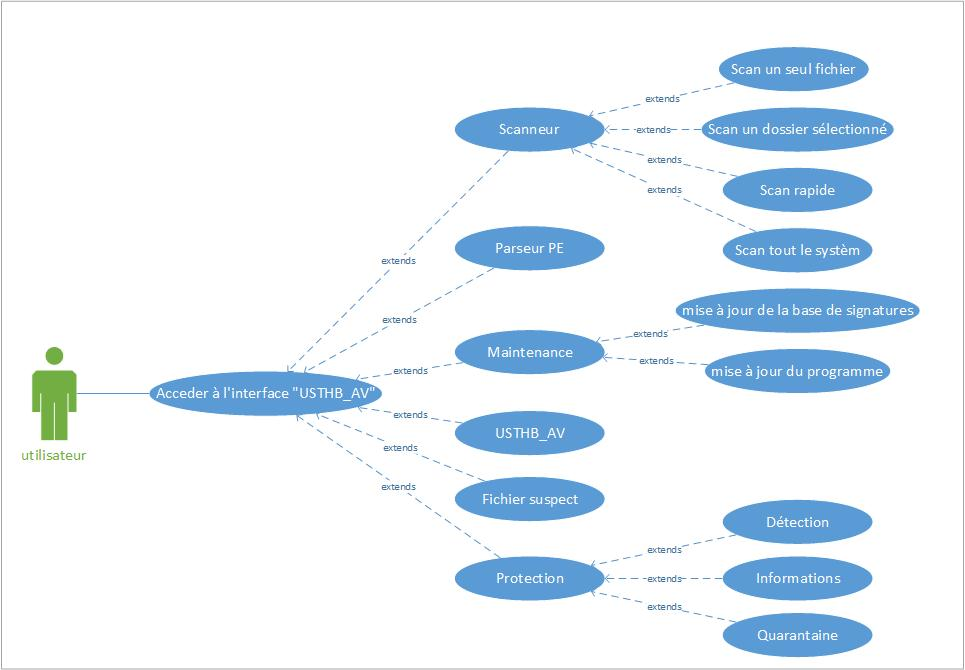
\includegraphics[scale=0.6]{Figures/antivirus.jpg}
\caption{Diagramme des cas d'utilisation de l'antivirus.}
\label{fig :mise} 
\end{center}
\end{figure}
\subsection{Parseur de PE}
\subsubsection{Objectif du parseur }
L'objectif de ce travail est d'observer le contenu d'un fichier exécutable. Avec ce parseur nous pouvons visualiser et examiner les fichiers de format PE ainsi que leurs structures internes (voire chapitre 2).\\


Le parseur PE sert à analyser les fichiers PE et d'autres usages différents. Il comporte un analyseur d'entête PE, une visionneuse des fonctions API importées, un testeur de validité du format PE, vérificateur et détecteur des packers.
\subsubsection{Vérifier  la validité d'un fichier PE}
Le test de validité d'un fichier de format PE, se fait selon les  étapes suivantes :
\begin{itemize}
\item Vérifier que le fichier a un entête DOS-MZ valide en comparant le premier WORD du fichier avec la valeur IMAGE\_DOS\_SIGNATURE qui doit être égale à "MZ";
\item Si le fichier a un entête DOS valide, on utilise la valeur contenue dans le champs \_lfanew pour trouver l'entête PE;
\item Comparer le premier DWORD de l'entête PE avec la valeur IMAGE\_NT\_SIGNATURE qui doit être égale à "PE00". Si les deux valeurs concordent, alors on peut considérer le fichier comme un fichier potentiellement valide.
\end{itemize}
L'organigramme suivant montre le test de validité d'un fichier PE :
\begin{figure}[H]
\begin{center}
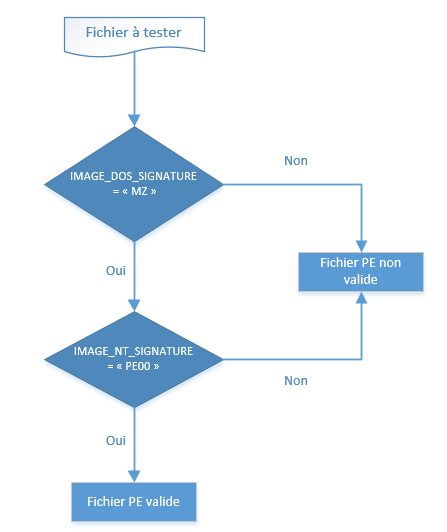
\includegraphics[scale=0.6]{Figures/org.PNG}
\caption{Test de validité d'un fichier PE.}
\label{fig :org} 
\end{center}
\end{figure} 
\subsubsection{Visualiser le contenu d'un fichier PE}
Dans cette étape nous affichons les informations internes du fichier PE, le nombre de sections, ses détails et quelques caractéristiques de ce dernier.
\begin{itemize}
\item Entry point : récupérer l'adresse mémoire où  sera chargé le fichier PE;
\item Détail PE   : afficher les caractéristiques du fichier PE et toutes les informations nécessaires pour charger ce  fichier en mémoire (citées dans la section 2.3.4 et  2.3.5 , chapitre 2);
\item Les sections PE : afficher les sections du fichier PE et leurs détails (cités dans la section 2.3.6 de chapitre 2).
\end{itemize}
\subsubsection{La table d'importation}
Afficher les DLL importées par le fichier PE après avoir chargé en mémoire, lister, pour chaque DLL, les fonctions utilisées (voir la section  2.3.7 et 2.3.8, chapitre 2).
\subsubsection{Détection des packers}
Enfin, nous examinons si le fichier PE est pacqué (voir la section 2.4 de chapitre 2 )  ou non, en utilisant une liste noire :
\begin{itemize}
\item La détection se fera au moyen d'un test de l'existence des noms de sections de fichier PE dans une liste noire des fonctions, les plus utilisées dans la compression. Si la fonction existe dans la liste, le fichier est conséquemment pacqué avec cette dernière, \end{itemize}
\subsection{Scanneur de malwares }
\subsubsection{Objectifs}
L'objectif de l'antivirus est tacitement de détecter les malwares avant leur exécution en mémoire, rechercher sur disque dur toute indication des malware; l'antivirus fonctionne en mode statique (voir la section 1.4.2.1, chapitre 1).
\subsubsection{Mécanismes de détection }
Pour atteindre cet objectif, nous devons étudier  les techniques anti-virales utilisées dans le mode de fonctionnement statique, recherche par signature, analyse spectrale et le contrôle d'intégrité (voir la section 1.4.3, chapitre 1). Le tableau~\ref{comp} montre une comparaison entre ces trois techniques :
\begin{table}[H]
\begin{tabular}{|p{4.5cm}|p{5cm}|p{5cm}|}
\hline \textbf{Technique} &  \textbf{Avantages} & \textbf{Inconvénients}\\
\hline \textbf{Recherche par signature} & détecter les malwares avant leurs exécutions en
mémoire & n'est pas capable de détecter les nouveaux malwares\\
\hline \textbf{Analyse spectral} & permet de détecter des nouveaux malwares & génère trop de faux positif \\
\hline \textbf{Contrôle d'intégrité}& permet de détecter les modifications de fichiers sur le disque & génère trop de faux positif \\
\hline
\end{tabular}
\caption{Comparaison entre les techniques anti-virales}
\label{comp}
\end{table}


D'après cette comparaison nous préférons la  recherche par signature, car elle répond avantageusement et favorablement à notre objectif.
\subsection{Composants du moteur antivirus}
\subsubsection{Base de signatures}
La base de signatures référence des dizaines de milliers de malwares, elle doit être mise à jour fréquemment pour reconnaître les nouveaux programmes malveillants~\cite{viruslist}.\\

La base de données d'un antivirus est un conteneur servant à stocker  l'ensemble des  signatures de malwares reconnus par l'antivirus pour être une référence de scan, cette base de signatures a plusieurs caractéristiques : type de la base de données, type et format des signatures et la façon de sa mise à jour.
\subsubsection{Type de la base de données}
Nous pouvons extraire des données de diverses bases de données, comme Microsoft Office Access, Microsoft SQL Server, les services OLAP de Microsoft SQL Server, de classeurs Excel et de fichiers de texte.\\


D'après le type et le format des signatures de l'antivirus, qui est un format texte, notre base de signatures sera une base de données orientée texte.\\

Une base de données orientée texte (ou "Base de données dans un fichier plat", de l'anglais "Flat file database") est un modèle de base de données (qui se présente,généralement, sous forme d'une table) sous la forme d'un simple fichier (formats .txt, .ini ,...).\\


Un fichier plat est un fichier texte contenant généralement un seul enregistrement par ligne, cet enregistrement est la signature de malware, chaque ligne de ce fichier texte correspond à une signature.\\

Le choix des fichiers plats se fait à seule fin de stocker les signatures des malwares, on n'a pas fait recours à une base de données "sql" car il n'y a pas d'avantages réels en faveur de l'utilisation de celle-ci et comprend mêmement de façon certaine quelques désavantages. Pour les actions standards (visualiser, éditer, ...), conserver l'information dans des fichiers plats est clairement plus rapide que d'y accéder au moyen d'une base de données. Sachant que l'avantage est essentiellement basé sur la simplicité, facilité de déploiement, légèreté et la non nécessité de dépendre d'un SGBD.
\subsubsection{Type de signature }
La technique anti-virale utilisée par notre antivirus pour détecter les malwares est la détection par signature "scanning", qui peut s'exprimer sous plusieurs types tels que : hash de malware et suite hexadécimale, cette  dernière est récupérée depuis le code  binaire du malware.
\begin{itemize}
\item \textbf{Hash de fichier : }une fonction de hachage (parfois appelée fonction de condensation) est une fonction permettant d'obtenir un condensé (appelé aussi condensat ou haché ou en anglais message digest) d'un texte, c'est-à-dire une suite de caractères assez courte représentant le texte qu'il condense. La fonction de hachage doit être telle qu'elle associe un seul haché à un texte en clair (cela signifie que la moindre modification du document entraîne la modification de son haché). D'autre part, il doit s'agir d'une fonction à sens unique (one-way function) afin qu'il soit impossible de retrouver le message original à partir du condensé. S'il existe un moyen de retrouver le message en clair à partir du haché~\cite{hashage}.\\

Les algorithmes de hachage les plus utilisés actuellement sont :\\


\begin{list}{•}{}

\item \textbf{Hash MD5}(Message Digest) : Développé par Rivest en 1991, MD5 crée une empreinte digitale de 128 bits à partir d'un texte de taille arbitraire en le traitant par blocs de 512 bits. Il est courant de voir des documents en téléchargement sur Internet accompagnés d'un fichier MD5, il s'agit du condensé du document permettant de vérifier l'intégrité de ce dernier~\cite{sha}.\\

Exemple  pour md5 : \textbf{e1ade9d04ad99dd70ec25b83841d8b72}\\


\item \textbf{SHA}(Secure Hash Algorithm) : pouvant être traduit par Algorithme de hachage sécurisé, SHA crée des empreintes d'une longueur de 160 bits. SHA-256 est une version améliorée de SHA, SHA-256 devient en 2002 un standard fédéral de traitement de l'information (FIPS du NIST). Elle produit un hachage de 256 bits~\cite{sha}.\\
Exemple pour sha1 : \textbf{2fd4e1c67a2d28fced849ee1bb76e7391b93eb12}\\
\newpage
En 2004, une équipe chinoise a découvert des collisions complète "même résultat d'hachage pour deux fichier différant", md5 n'est donc plus considère comme sûr au sens cryptographie, et il est recommander d'utiliser la fonction sha256 qui est plus fiable pour notre signature~\cite{shamd}.\\


\end{list}
\item \textbf{Suite hexadécimale : }la signature est une suite hexadécimale récupérée depuis le code binaire de malware, d'une taille variable et un offset différent, il faut que le malware soit bien identifié par cette suite.  
\end{itemize}
\subsubsection{Choix du type de signature}
\textbf{Quel est le type le plus fiable et rapide pour le bon fonctionnement de l'antivirus ?}\\
Pour répondre à cette question, nous faisons une expérience par rapport aux points suivants : nombre de malwares détectés, temps de détection, faux positif et nombre de malwares polymorphes détectés, par rapport à une base du 7404 signatures, en plaçant 10 malwares dans un dossier qui contient 50 fichiers sains, et pour tester l'efficacité de détection des malwares polymorphes par les deux types de signature, nous ajoutons quatre malwares modifiés avec l'éditeur Hexadécimal HxD, en gardant toujours leur   fonctionnement, le volume de données analysées est de 4.2 G, à la fin de cette expérience nous avons obtenu les résultats indiqués dans le tableau~\ref{signatures} : 
\begin{table}[H]
\begin{center}
\begin{tabular}{|p{3cm}|p{2cm}|p{3cm}|p{2cm}|p{2cm}|}
\hline Type de signature &  malwares détectés & Temps de détection & Faux positifs & Malwares polymorphes\\
\hline Hashage de Fichier & 10 & 04:23:12:34 & 0 & 0 \\
\hline Suite hexadécimal & 15 & 00:01:34:01 & 1 & 4 \\
\hline
\end{tabular}
\caption{Comparaison entre les types de signatures}
\label{signatures}
\end{center}
\end{table}
\textbf{\textit{Analyse des résultats }}
\begin{itemize}
\item Hashage de fichier : dix malwares détectés, pas de faux positif et aucun malware polymorphe n'a été détecté dans un temps dépassant de quatre heures 
\item Suite hexadécimal : onze malwares détectés, un faux positif et quatre malwares polymorphes détectés dans un temps très court. \\


D'après les résultats obtenus, nous préférons utiliser la suite hexadécimale pour notre signature car elle nous permet de détecter tous les malwares "10 malware", ainsi que les malwares polymorphes, mais avec un seul Faux positif, dans un temps inférieur à ce de type hachage fichier qui ne nous permet pas à détecter les malwares polymorphes. 

\end{itemize}
\newpage
\subsubsection{Format de signatures}
Le format de signature est le suivant :\\
\begin{table}[H]
\begin{center}
\begin{tabular}{|p{3.5cm}|p{3.5cm}|p{3.5cm}|p{3.5cm}|}
\hline Offset & Suite hexadécimale &  Nom de malware & Type de malware \\
\hline
\end{tabular}
\caption{Format de signatures}
\label{signatures}
\end{center}
\end{table}

\begin{itemize}
\item \textbf{Offset : }l'offset d'où la suite hexadécimale a été récupéré  
\item \textbf{Suite hexadécimale : }une suite d'octets récupérés depuis le code du malware 
\item \textbf{Nom de malware : }nom de malware attribue par les éditeurs de l'antivirus 
\item \textbf{Type de malware : }virus, worm, cheval de troie, ...
\end{itemize} 
Ex : 58ab|38896E0E41B0CB35F3D7B94D6D973F143A75CD97F974A514869E1 : Conficker/Worm

\subsubsection{La mise à jour}
L'efficacité des solutions antivirus dépend des bases de signatures de définitions du malware. Ces bases sont dynamiques intrinsèquement,et ce, étant donné l'activité des auteurs de malware. Par exemple, les analystes viraux de Kaspersky Lab détectent et ajoutent cent nouvelles menaces, quotidiennement, à la base de l'antivirus~\cite{mise}.\\


Néanmoins, une mise à jour régulière de la protection antivirus est plus importante que jamais, étant donné la rapidité avec laquelle les menaces actuelles sont capables de se propager. Les éditeurs d'antivirus ont réduit l'intervalle entre les mises à jour de signatures de façon trimestrielle à une façon mensuellement et finalement à une façon quotidienne.\\


Désormais, Kaspersky Lab fournit les mises à jour de définitions virus toutes les heures.
Et pour cela, nous proposons pour notre antivirus deux méthodes pour le mettre à jour, l'une est \textbf{automatique} et l'autre \textbf{manuelle} déclenchée de la part de l'utilisateur.\\


Dans les deux cas, la mise à jour sera effectuée selon les étapes suivantes :

\begin{itemize}
\item Télécharger un fichier nommé "info.txt" depuis "Github"
\item Récupérer un hash de la base de signatures de site web depuis ce fichier téléchargé 
\item Comparaison entre le hash récupéré de fichier "info.txt" et le hash de la base de signatures actuel, si les deux hash sont identiques alors l'antivirus informe l'utilisateur que sa base virale est à jour, sinon nous effectuons les tâches suivantes:
\begin{list}{•}{}
\item Télécharger un fichier texte depuis le site de l'antivirus nommé "new\_bdd\_mal.txt" 
\item Remplacer l'ancienne base de signatures par la nouvelle 
\item Informer l'utilisateur que la mise à jour est bien terminée.

\end{list}

\end{itemize}

Le diagramme suivant montre les étapes pour faire la mise à jour de notre antivirus :
\begin{figure}[H]
\begin{center}
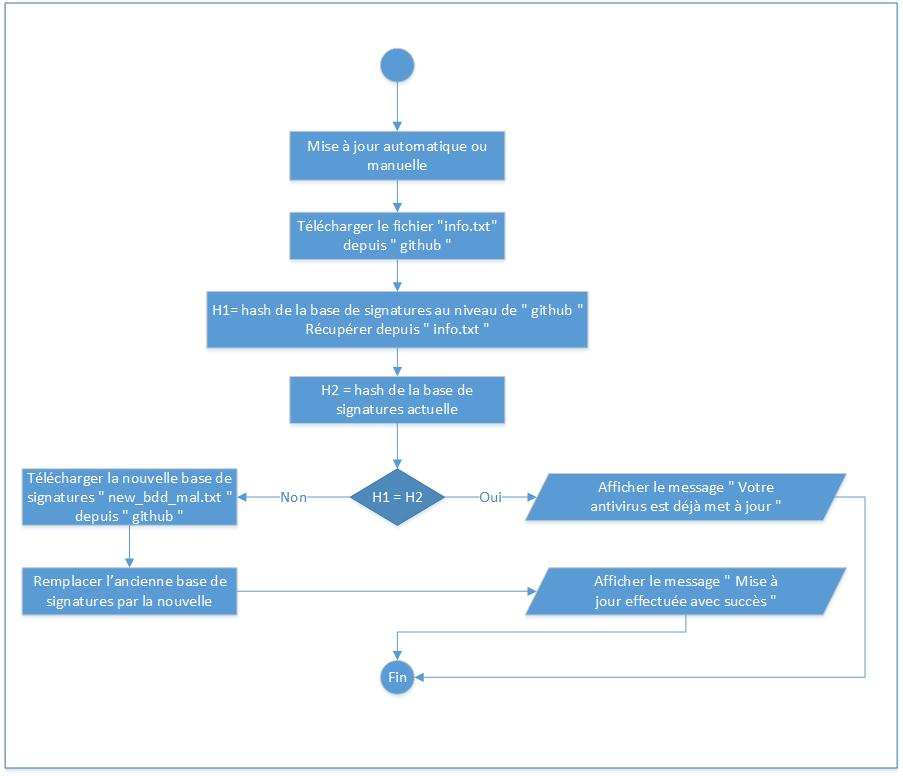
\includegraphics[scale=0.6]{Figures/mise.jpg}
\caption{Les étapes de la mise à jour de l'antivirus.}
\label{fig :scan} 
\end{center}
\end{figure}


\subsubsection{Les types de scan} 
L'antivirus examine (scan) le système à la demande : un fichier, un dossier ou tous les fichiers du disque. Un scan complet consomme beaucoup de ressources matérielles et du temps, mais il est conseillé de le faire de temps en temps.\\


Dans cette partie, nous allons proposer quatre manières pour effectuer un scan :\\

\begin{itemize}
\item Scan un seul fichier : il effectue une analyse d'un seul fichier sélectionné  
\item Scan un dossier sélectionné : il effectue une analyse d'un répertoire  sélectionné  
\item Scan rapide : il effectue uniquement une analyse rapide du disque system "C:\ de l'ordinateur", seulement les fichiers aux extensions perceptibles à une infection (.exe, .ocx, .dll, .cpl) seront testés
\item Scan tout le système : il effectue un scan de tous les disques de l'ordinateur.

\end{itemize}
\subsubsection{La présentation des résultats d'analyse}
Après avoir effectué un scan selon l'un des types cités précédemment, les résultats de scan seront présentés à l'utilisateur dans une grille, pour chaque type de scan, le rapport comportera les champs suivant :
\begin{itemize}

\item Nom du malware : un nom attribué par les éditeurs des malwares
\item Type : c'est le type de malware (section 1.3.2, chapitre 1)
\item Chemin : le chemin courant du malware détecté.  

\end{itemize}
\subsection{Autres fonctionnalités }
\begin{itemize}
 
\item La langue d'utilisation : dans cette option, nous offrons à l'utilisateur la possibilité de choisir la langue,  nous  proposons  deux langues : Anglais et Français 
\item Information sur la protection : cette fonctionnalité permet à l'utilisateur de visualiser  des informations concernant l'état actuel de l'antivirus comme :
\begin{list}{•}{}
\item La liste des malwares détectés  par notre antivirus classés par leur nom et type 
\item Informations sur la base de signatures telles que sa taille "nombre de signatures", le nombre des virus et la version actuelle de l'antivirus
\item Quarantaine : cette fonctionnalité permet d'accéder au dossier quarantaine, visualiser son contenu.
\end{list}

\item L'accès au site officiel de l'antivirus : permet à l'utilisateur de découvrir les fonctionnalités de l'antivirus, et les éventuels problèmes pouvant être rencontrés durant l'utilisation, télécharger le guide d'utilisation et actualités concernant la sécurité informatique et bien évidemment, soumettre des questions.
\item Guide d'utilisation : un guide pratique expliquant la manière d'utilisation de l'antivirus et toutes ses tâches
\item Mise à jour de programme : effectuera selon les mêmes étapes de la mise à jour de la base de signatures virales, au lieu de télécharger la base de signatures, des fichiers ".dll" seront téléchargés
\item L'envoi d'un fichier suspect : permet à l'utilisateur d'envoyer un fichier suspect compressé, protégé par le mot de passe "infected" à l'équipe d'analyse de l'antivirus.
\end{itemize}
\section{La façon de présenter l'antivirus}
L'antivirus sera présenté au moyen d'une interface graphique, qui permettra de visualiser l'état actuel de la protection, modifier la langue, effectuer manuellement un scan et d'utiliser l'outil parseur PE pour avoir des détails techniques concernant un fichier PE, l'accès à cette interface peut se faire selon trois manières différentes :
\begin{itemize}
\item A partir d'un raccourci, qui permet d'appeler l'interface de l'antivirus
\item A partir de l'icône de l'antivirus présentée dans la zone de notification "systray", en bas à droite de l'écran près de l'horloge par un simple clic
\item A partir du menu Démarrer, par un clic sur Programmes suivi par la sélection du nom d'antivirus. \\
\end{itemize}
L'antivirus se lance automatiquement au démarrage de Microsoft Windows.
\section{Fonctionnement de  l'antivirus :}
D'après cette conception, notre antivirus a deux tâches essentielles et primordiales, un parseur PE est un outil de scan
\subsection{Parseur PE }
L'utilisateur sélectionne un fichier depuis le système ou les disques amovibles pour afficher ses détails techniques, par un simple clic sur un bouton appelé "Parseur PE" qui permet d'accéder à une nouvelle page et un nouveau bouton " ... ", ce dernier permet d'accéder aux différents disques de votre système pour choisir un fichier par un clic sur le nom de fichier sélectionné, suivi d'une validation du choix avec le bouton "OK", les résultats de l'analyse seront affichés dans une fenêtre graphique, ainsi que le chemin de fichier sélectionné.
\subsection{Scanneur de malwares}
\subsubsection{phase de scan}
L'utilisateur sélectionne un type de scan, à savoir; scan rapide, scan d'un seul fichier, scan d'un dossier sélectionné ou un scan de tout le système, ensuite l'antivirus analysera  les fichiers relatifs au scan sélectionné, et ce, comme suit :\\

\begin{itemize}
\item Parcourir la base de signatures, pour chaque signature, nous testons leur apparence dans le code binaire de fichier testé selon les étapes suivantes : \\
\begin{list}{•}{}
\item Récupérer un offset depuis la signature testée
\item Récupérer la suite hexadécimale relative a l'offset récupéré, depuis le code binaire du fichier testé
\item Comparer la suite de la signature testé avec la suite récupérée.
\end{list}
\item Si les deux suites comparées sont identiques, nous sommes devant deux versions :
\begin{list}{•}{}
\item Scan d'un seul fichier : le fichier est signalé comme malware, et c'est la fin de scan
\item Autre type de scan : le fichier est signalé comme malware, ce qui nécessite la ré-exécution des étapes de scan dès le début pour le fichier suivant.
\end{list}
\item Si les deux suites comparées sont différents, nous testons la signature qui suit et ainsi de suite, à la fin de cette opération, si aucune signature n'a été trouvée; on est devant deux cas :
\begin{list}{•}{}
\item Scan d'un seul fichier : fin de scan
\item Autre type de scan : ce qui nécessite de refaire les étapes de scan dès le début pour le fichier suivant.\\
\end{list}
\end{itemize}

Le diagramme suivant montre les étapes de scan:
\begin{figure}[H]
\begin{center}
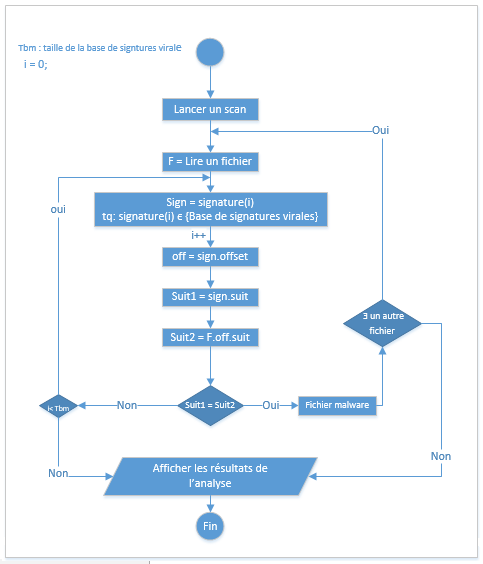
\includegraphics[scale=1]{Figures/scans.jpg}
\caption{Diagramme des étapes de scan.}
\label{fig :mise} 
\end{center}
\end{figure}
\subsubsection{Traitement des résultats de scan }

Après la détection d'un malware, nous proposons les actions suivantes :
\begin{itemize}
\item \textbf{Supprimer : }permet de supprimer le fichier signalé comme malware depuis son emplacement d'origine;  
\item \textbf{Mettre en Quarantaine : }si le fichier signalé ne peut ou ne doit pas être supprimé (fichier sensible, document personnel) alors il sera isolé jusqu'à une éventuelle opération, l'isolation se fait dans un dossier nommé  "quarantaine" 
\item \textbf{Ne rien faire : }Si aucune action n'est souhaitable, le fichier est ignoré.\\
\end{itemize} 
\section{Gestion de la base de signatures virales}
La détection d'un nouveau malware se fera par les éditeurs d'antivirus ou par un signalement (l'utilisateur envoie le malware compressé avec le mot de passe de décompression) de la part des utilisateurs, une fois détecté le malware sera analysé pour identifier son nom, son type,  son fonctionnement et son objectif.\\

    
Après la phase d'analyse, nous allons attribuer une signature de détection à ce malware, qui lui est propre, la génération de la signature virale commence par la récupération  de la suite hexadécimale qui identifie de manière unique le malware, suivie par l'association de l'offset, nom et du type de malware à cette suite.\\


Pour chaque nouveau malware détecté, nous devons mettre à jour la base de signatures virales, cette mise à jour  comporte plusieurs tâches qui sont gérées uniquement par les administrateurs d'antivirus, ces tâches sont :
\begin{itemize}

\item \textbf{Ajouter une signature : }permet à l'administrateur d'ajouter une nouvelle  signature à la base de signatures, l'ajout d'une signature se fait selon les étapes suivantes :
\begin{list}{•}{}
\item Sélectionner le malware à signer
\item Choisir l'offset de la suite hexadécimale à l'aide de parseur PE, l'offset peut être la valeur de l'EntryPoint ou l'offset de l'un des sections ".data", ".code", ...
\item Récupérer la suite relative à l'offset choisi
\item Tester l'apparence de cette suite dans la base de fichiers légitimes afin d'éviter les faux positifs pour la signature générée
\item Associer le nom et le type de malware qui ont été définis par l'analyste à la suite et l'offset généré. La génération d'une suite est terminée par l'insertion de cette dernière dans la base de signatures virale.\\ 
\end{list}
La figure~\ref{fig :generation} montre les étapes à suivre pour générer des signatures :
\begin{figure}[H]
\begin{center}
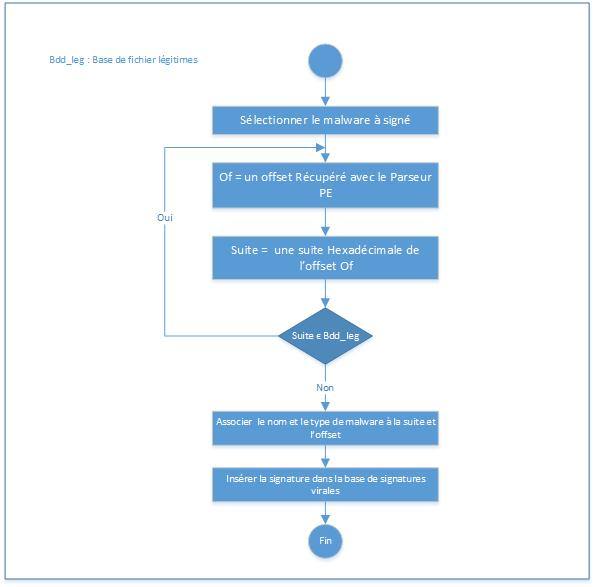
\includegraphics[scale=0.7]{Figures/generation.jpg}
\caption{Les étapes de génération d'une signature.}
\label{fig :generation} 
\end{center}
\end{figure}

\item \textbf{Afficher la base de signatures : }permet d'afficher le contenu de la base de signatures 
\item \textbf{Afficher la base de malwares : }permet de lister les noms de malwares
\item \textbf{Supprimer une signature : }supprime une signature identifiée par le nom de malware
\item \textbf{générer le fichier "info.txt" : } après chaque mise à jour, l'administrateur doit générer le fichier "info.txt" pour le charger sur GitHub. 
\end{itemize}


\section{Les faux positifs }
Pour éviter ou minimiser les faux positifs, nous allons construire une base de données des fichiers légitimes, qui présentent les fichiers fondamentaux d'une installation Microsoft Windows fraiche.\\

Et pour chaque signature virale générée, nous allons tester son apparence dans cette base des fichiers légitimes, si cette dernière existe, nous devons régénérer une autre signature, et ce, jusqu'à l'arrivée d'une signature qui n'existe plus. 

\subsection{Description de la base de fichiers légitimes}
La base des fichiers légitimes, comporte les fichiers déclarés par les éditeurs d'antivirus comme fichiers légitimes. Pour bien vérifier l'intégrité d'un fichier, nous utilisons la fonction d'hachage sha256, donc le fichier légitime sera stocké par son hash dans un fichier plat.
\subsection{Gestion de la base de fichiers légitimes}
Pour chaque nouveau fichier qui fait partie d'une nouvelle version Microsoft Windows ou mise à jour.l'administrateur met à jour la base de fichiers légitimes par l'insertion de ce fichier dans cette dernière, attribuer un nom au fichier qui est le hash de ce dernier .\\

Le diagramme de cas d'utilisation suivant donne une vision globale sur les tâches effectuées par l'administrateur d'antivirus.
\begin{figure}[H]
\begin{center}
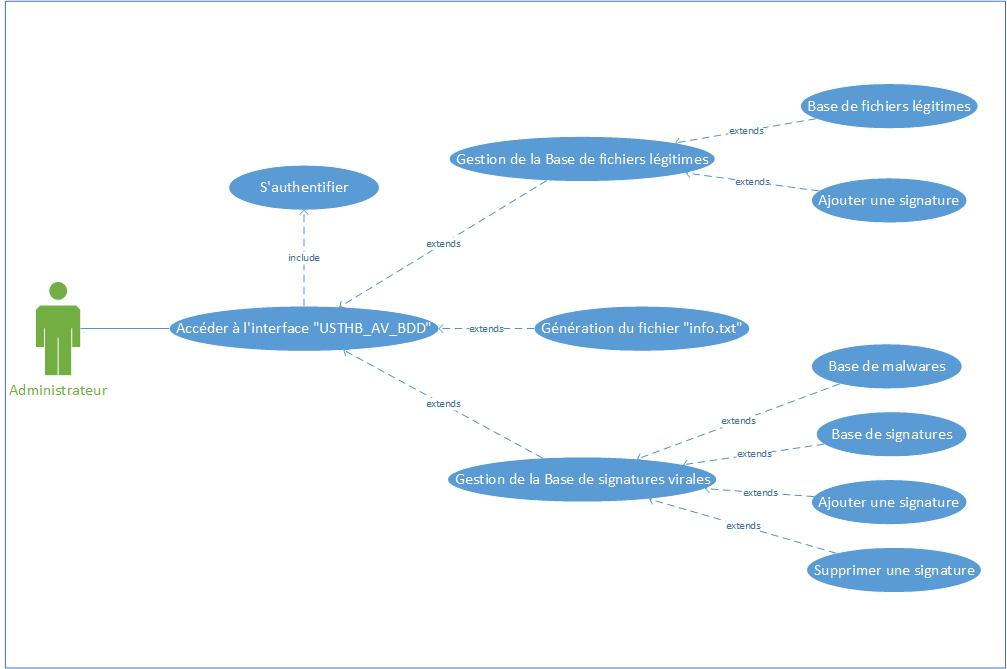
\includegraphics[scale=0.6]{Figures/Admin.jpg}
\caption{Détail de la gestion de la base de signatures.}
\label{fig :mise} 
\end{center}
\end{figure}

\section{Conclusion}
Dans ce chapitre, nous avons détaillé la conception de l'antivirus  qui est composée de deux outils, \textbf{un parseur PE} et \textbf{un Scanneur de malwares}.\\

Le parseur PE permet de visualiser les informations techniques d'un fichier PE et pour le scanneur, nous avons adopté la technique anti-virale de recherche par signature de type suite Hexadécimale, et pour éviter les faux positifs nous avons proposé une base de  signatures des fichiers légitimes.\\

 
Dans le chapitre suivant, l'implémentation de la solution anti-virale sera abordée.